\section{要素技術}
\subsection{ルーティングプロトコル}
AS(Autonomous System)とは,経路制御に関するルールを決めて,それをもとに運用する範囲を指す.
AS内部の経路制御ではIGP(Interior Gateway Protocol),AS間の経路制御ではEGP(Exterior Gateway Protocol)を用いる\cite[p.173]{マスタリングTCPIP}.
\subsubsection{経路制御アルゴリズム}
経路制御のアルゴリズムは大きく2つある.
\paragraph{距離ベクトル型}
距離と方向によってネットワークやホストの位置を決定し,これらの情報から経路制御表を作成する.
処理は比較的簡単だが,ルータ間で交換される情報は距離と向きだけなので,ネットワークが複雑になると,経路の収束\footnote{経路制御情報が安定すること.}に時間がかかる\cite[p.174\ -\ p.175]{マスタリングTCPIP}.
\paragraph{リンク状態型}
ルータがネットワーク全体の接続状態を理解して経路制御表を作成する方法.
ネットワークの構造は,どのルータにとっても同じなので,すべてのルータが同じ経路制御情報を持つ.
ルータ間の経路制御情報をすばやく同期させれば,経路制御を安定させられる.
リンク状態型は複雑なネットワークでも安定した経路制御をできるが,欠点としてネットワークトポロジーから経路制御表を作成する計算コストが高い\cite[p.175]{マスタリングTCPIP}.
\subsubsection{主なルーティングプロトコル}
主なルーティングテーブルと,方式について説明する.ここでは,RIPとOSPFを取り上げる.
\begin{center}
    \begin{tabularx}{\textwidth}{c|C|C|C}
        \hline
        分類     & \multicolumn{2}{c|}{IGP} & EGP              \\
        \hline
        プロトコル名 & RIP                      & OSPF   & BGP     \\
        \hline
        アルゴリズム & 距離ベクトル型                  & リンク状態型 & 距離ベクトル型 \\
        \hline
    \end{tabularx}
\end{center}
\paragraph{RIP}RIP(Routing Information Protocol)は,距離ベクトル型のルーティングプロトコルである.
経路制御情報を30秒周期でブロードキャストし,情報を伝搬する(\figref{fig:RIPの経路情報交換}).
距離が一番短い,つまりホップ数が最小になる経路を選択する\cite[p.276\ -\ p.277,\ p.132]{マスタリングTCPIP,インターネット工学}.
\begin{figure}
    \centering
    \begin{tikzpicture}
        \tikzset{dist/.style={midway,fill=red!10,text=black,align=center,text width=2cm,rounded corners}};
        \coordinate (ntA) at (0,0);
        \node[right=2.4cm of ntA](rt1){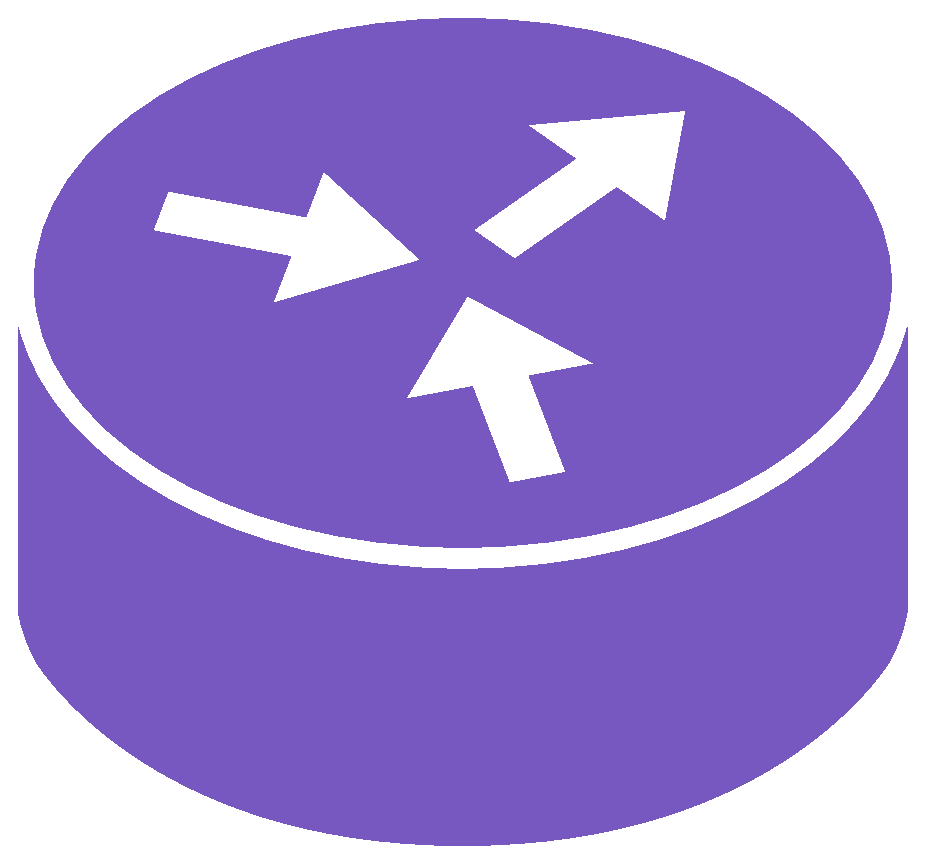
\includegraphics[keepaspectratio,width=2cm]{../network_iconset/router_01_nb.pdf}};
        \node[right=2.5cm of rt1](rt2){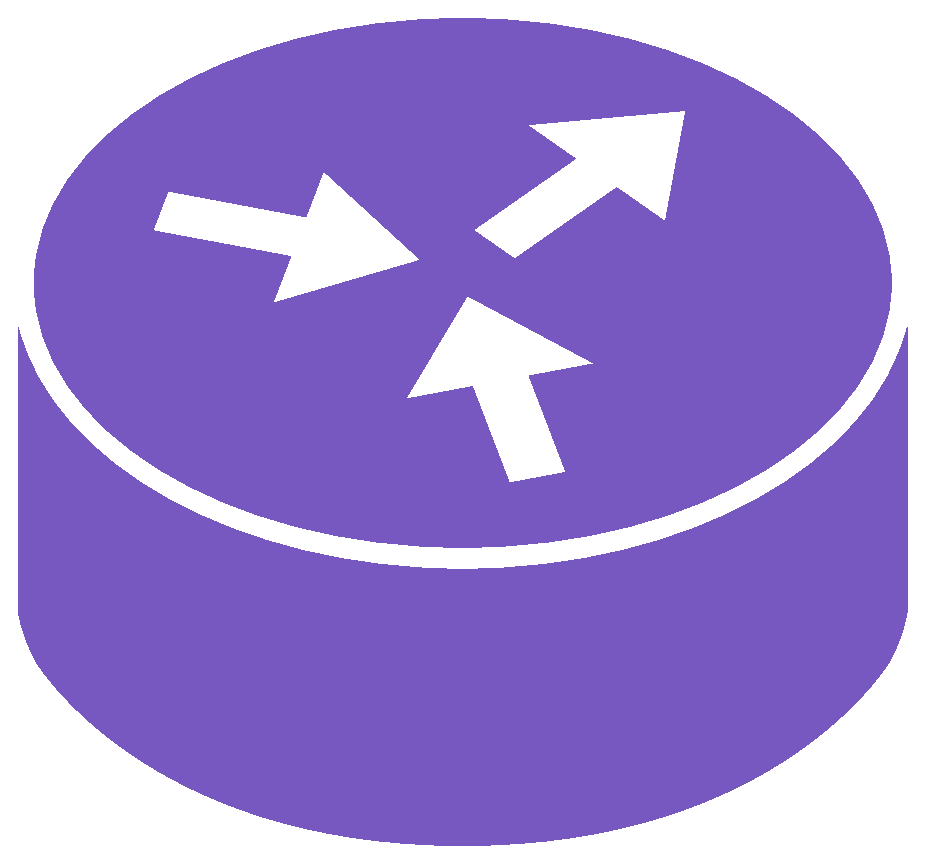
\includegraphics[keepaspectratio,width=2cm]{../network_iconset/router_01_nb.pdf}};
        \node[above=2cm of rt2](rt3){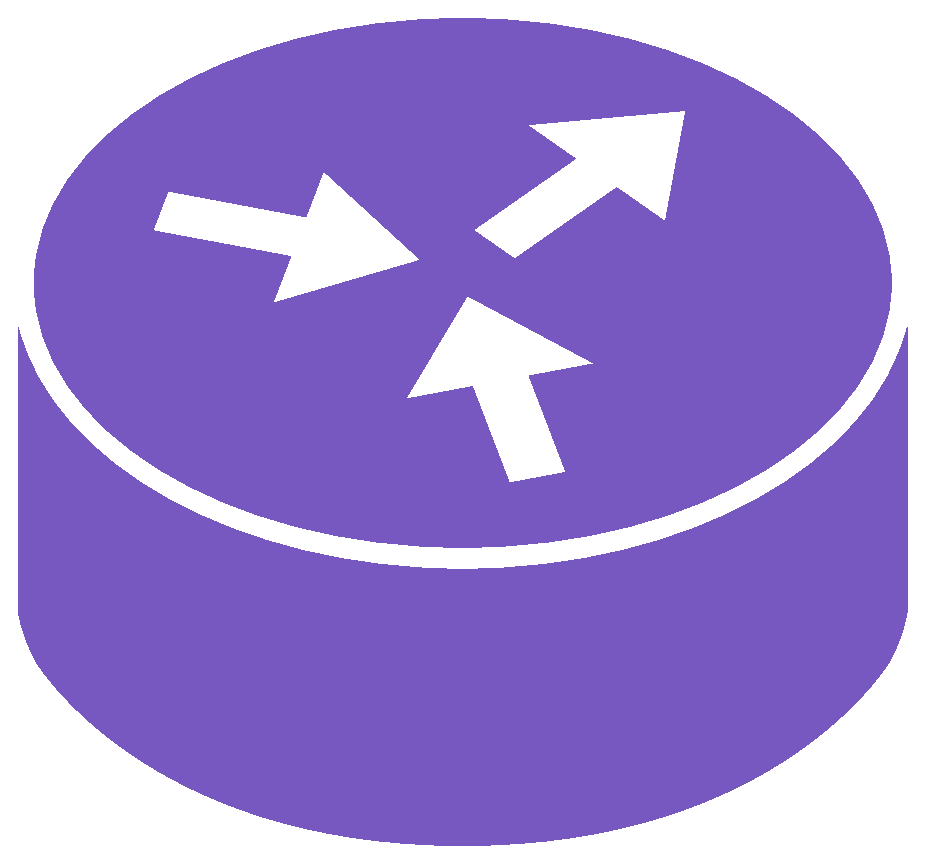
\includegraphics[keepaspectratio,width=2cm]{../network_iconset/router_01_nb.pdf}};
        \node[right=2.5cm of rt2](rt4){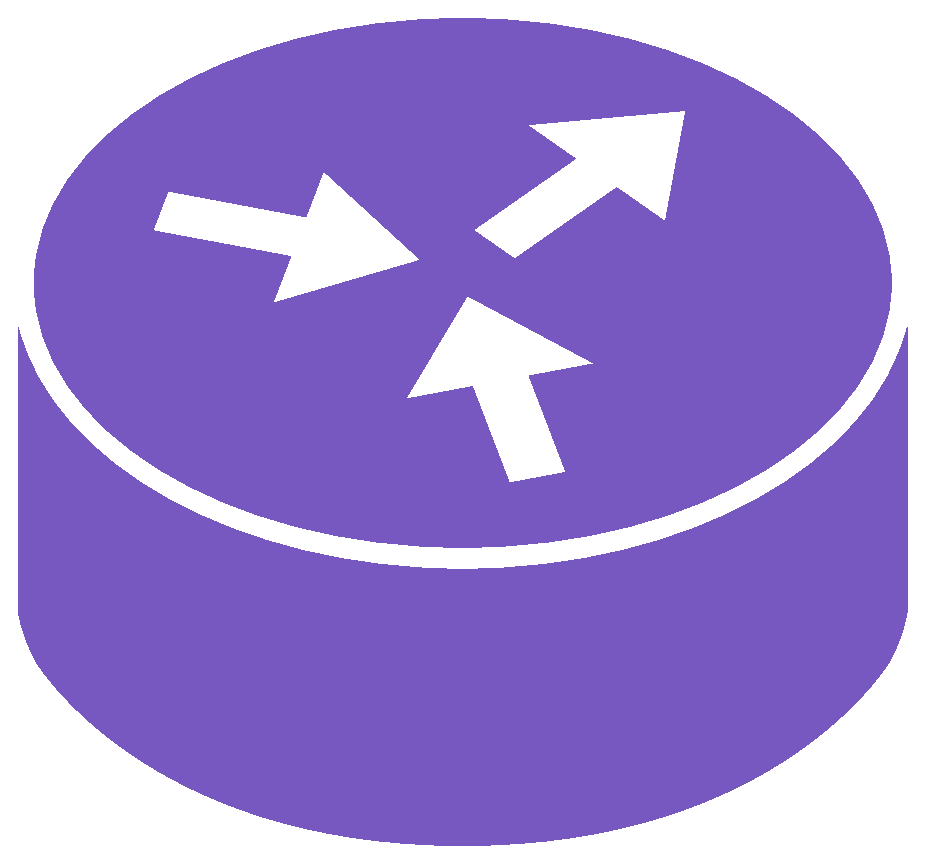
\includegraphics[keepaspectratio,width=2cm]{../network_iconset/router_01_nb.pdf}};
        \draw[ultra thick]{
            (ntA)--(rt1)node[midway,above]{Network1 (NW1)}
            (rt1)--(rt2)
            (rt2)--(rt3)
            (rt2)--(rt4)
            (rt3)-|(rt4)
            (rt3)--($(rt3.west)+(-1cm,0cm)$)
        };
        \foreach \u in{1,2,...,4}{
                \node[below=.2cm,text=white]at(rt\u){ルータ\u};
            }
        \draw[dashed,red!80!black,thick,-latex]($(rt1.east)+(0,-.2cm)$)--($(rt2.west)+(0,-.2cm)$)node[dist,below=.2cm]{\scriptsize ルータ1はNW1まで距離1};
        \draw[dashed,red!80!black,thick,-latex]($(rt1.west)+(0,-.2cm)$)--(0,-.2cm);
        \draw[dashed,red!80!black,thick,-latex]($(rt2.north)+(-.2cm,0cm)$)--($(rt3.south)+(-.2cm,0cm)$)node[dist,left=.2cm]{\scriptsize ルータ2はNW1まで距離2};
        \draw[dashed,red!80!black,thick,-latex]($(rt3.east)+(0cm,-.2cm)$)-|($(rt4.north)+(-.2cm,0cm)$)node[dist,below left=.2cm]{\scriptsize ルータ3はNW1まで距離3};
        \draw[dashed,red!80!black,thick,-latex]($(rt2.east)+(0,-.2cm)$)--($(rt4.west)+(0,-.2cm)$)node[dist,below=.2cm]{\scriptsize ルータ2はNW1まで距離2};
        \draw[dashed,red!80!black,thick,-latex]($(rt4.north)+(.2cm,0cm)$)|-($(rt3.east)+(0,.2cm)$)node[dist,right=.2cm]{\scriptsize ルータ4はNW1まで距離3};
    \end{tikzpicture}
    \caption{RIPの経路情報交換}
    \label{fig:RIPの経路情報交換}
\end{figure}
\paragraph{OSPF}
OSPF(Open Shortest Path First)は,リンク状態型のルーティングプロトコルで各リンクに重みをつけ,この重みが最小となるような経路を選択する.
ホップ数が最小でなくても,コストが最小の経路を選択する.
\figref{fig:OSPFでの経路選択}の例では,ホップ数が最小の経路はInternet VPNでのコストが大きいため,コストが最小となる経路を経路を選択している.
OSPFのコスト算出は,最大通信帯域が大きいほど小さな値が設定される\cite[p.138]{インターネット工学}.
\begin{figure}
    \centering
    \begin{tikzpicture}
        \node(hostA){
\includegraphics[keepaspectratio,width=2cm]{../network_iconset/laptop_nb.pdf}};
        \node[right=1cm of hostA](rtA){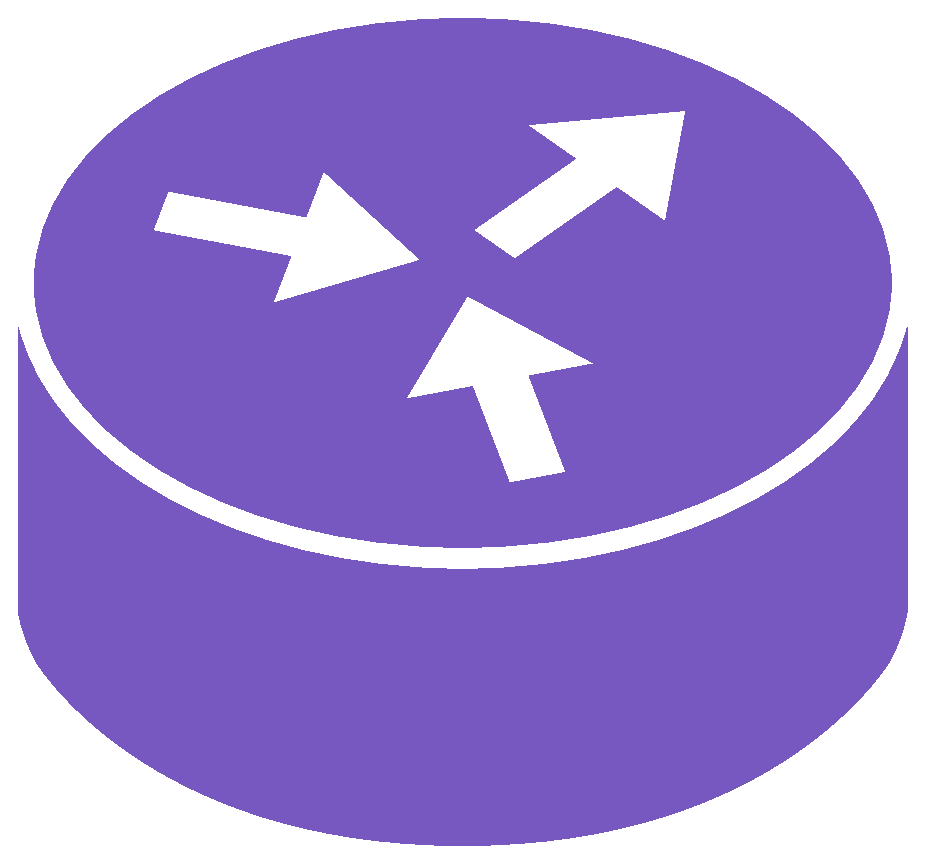
\includegraphics[keepaspectratio,width=2cm]{../network_iconset/router_01_nb.pdf}};
        \node[below=1cm of rtA](rtB){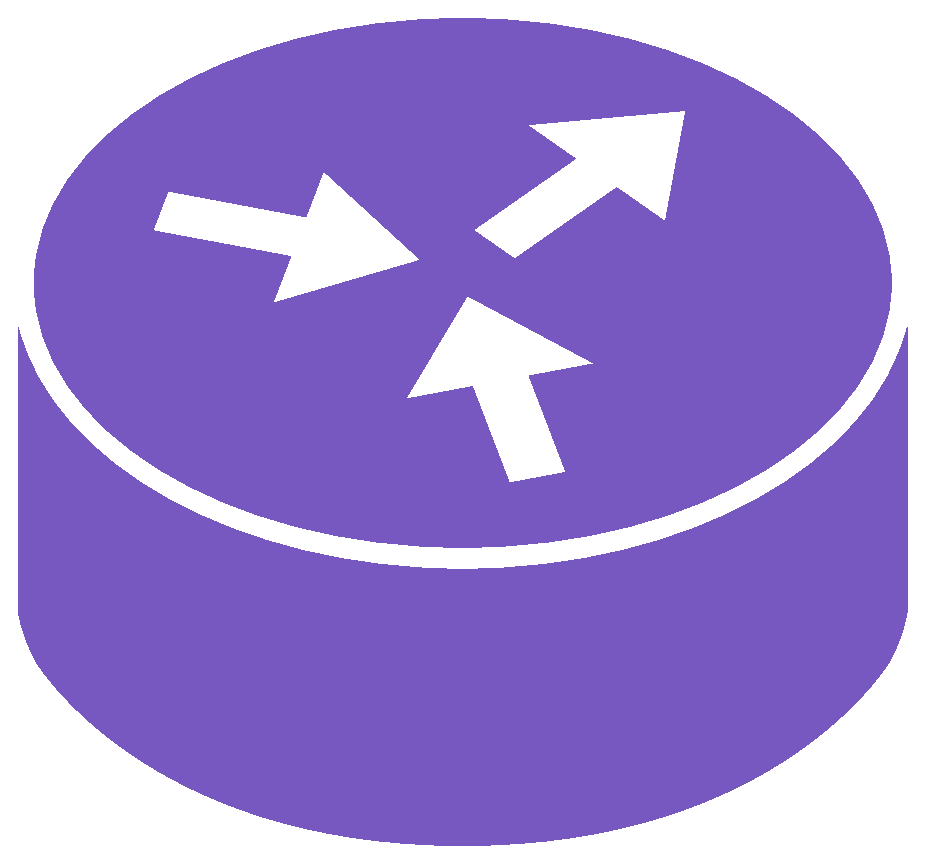
\includegraphics[keepaspectratio,width=2cm]{../network_iconset/router_01_nb.pdf}};
        \node[right=4cm of rtB](rtE){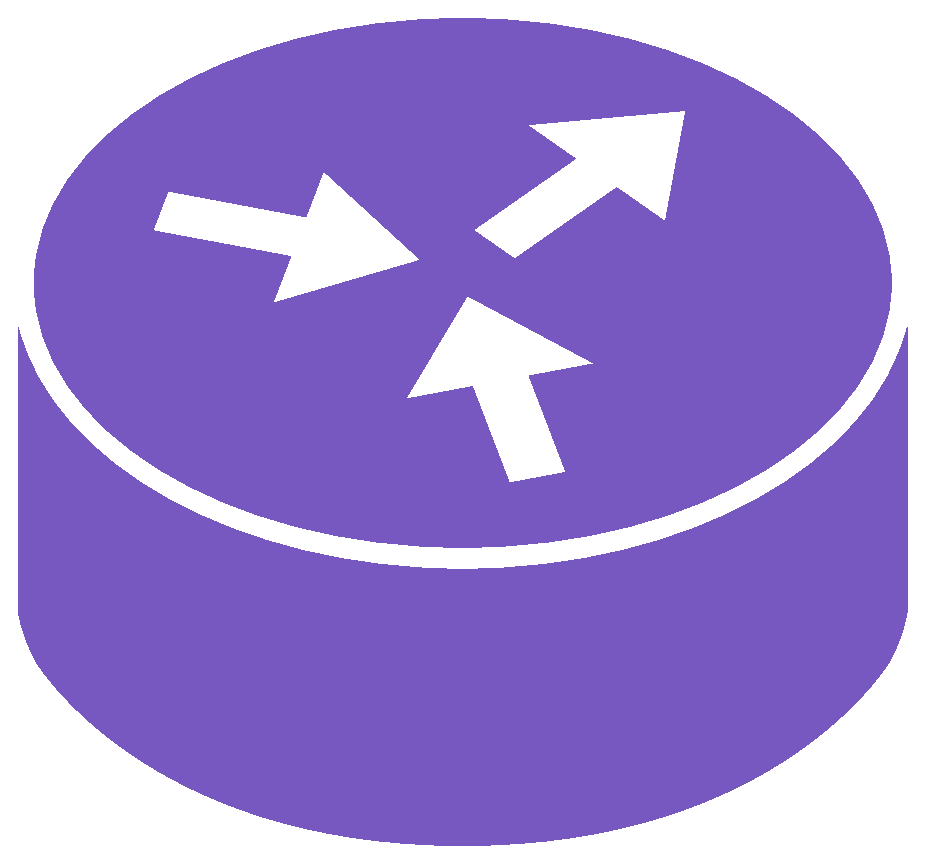
\includegraphics[keepaspectratio,width=2cm]{../network_iconset/router_01_nb.pdf}};
        \node[above=1cm of rtE](rtD){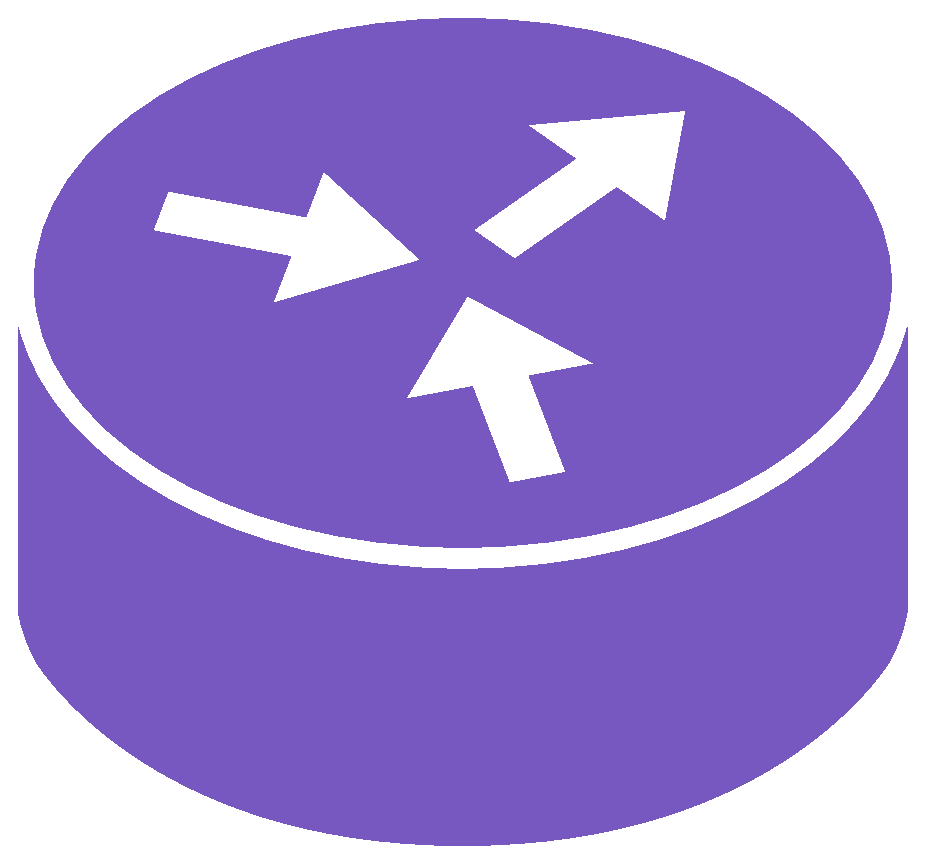
\includegraphics[keepaspectratio,width=2cm]{../network_iconset/router_01_nb.pdf}};
        \node[right=1cm of rtD](hostB){
\includegraphics[keepaspectratio,width=2cm]{../network_iconset/laptop_nb.pdf}};
        \node[anchor=south](rtC) at($(rtA)!0.5!(rtD)+(0,1.5cm)$){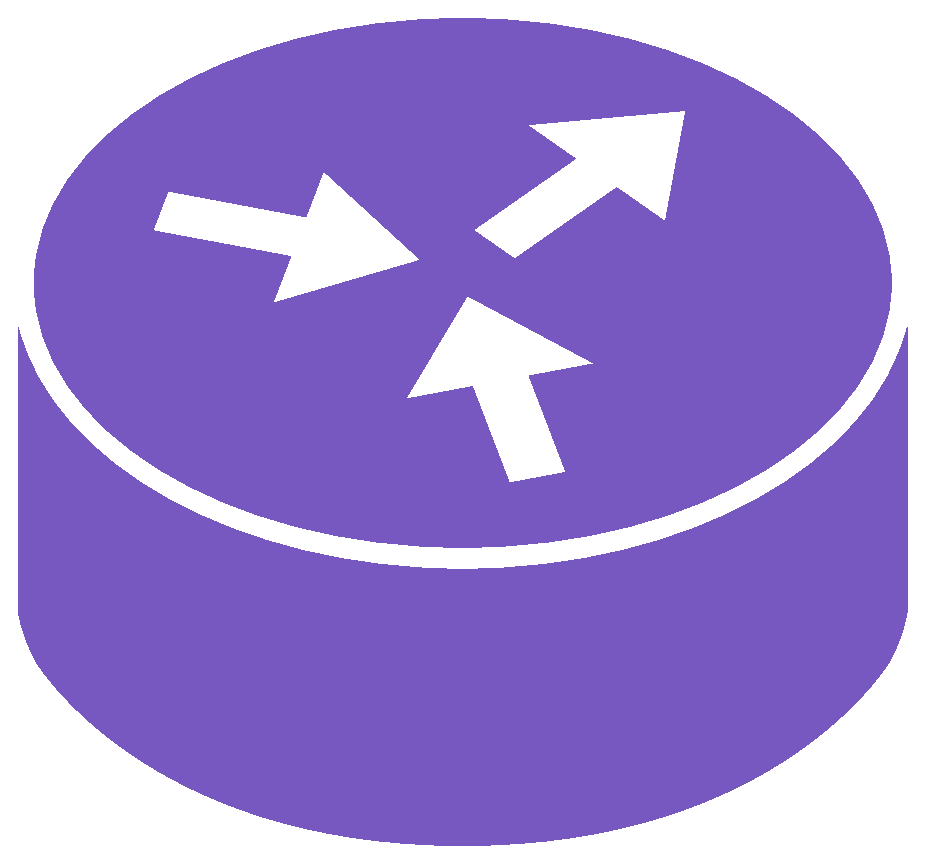
\includegraphics[keepaspectratio,width=2cm]{../network_iconset/router_01_nb.pdf}};
        \coordinate (a) at ($(rtA)!0.5!(rtB)$);
        \coordinate (b) at ($(rtD)!0.5!(rtE)$);
        \draw[ultra thick]{
            (hostA)--(hostA|-a)
            ($(hostA|-a)+(-.5cm,0)$)--($(a)+(.5cm,0)$)node[midway,align=center](la1){}
            (hostB)--(hostB|-b)
            ($(hostB|-b)+(.5cm,0)$)--($(b)+(-.5cm,0)$)node[midway,align=center](la2){}
            (rtA)--(a)
            (rtB)--(a)
            (rtD)--(b)
            (rtE)--(b)
        };
        \draw[ultra thick,densely dashed]{
            (rtA)|-(rtC)node[rounded corners,text opacity=1,fill opacity=.5,text width=3cm,fill=cyan!30,midway,align=center,left=-.4cm]{\scriptsize 広域インターネット網\\100Mbps\\コスト\(=100\)}
            (rtC)-|(rtD)node[rounded corners,text opacity=1,fill opacity=.5,text width=3cm,fill=cyan!30,midway,align=center,right=-.4cm]{\scriptsize IP-VPN網\\200Mbps\\コスト\(=90\)}
        };
        \draw[ultra thick,dash dot]{
            (rtB)--(rtE)node[rounded corners,text width=3cm,text opacity=1,fill opacity=.5,above=.1cm,fill=magenta!30,midway,align=center]{\scriptsize Internet VPN\\50Mbps\\コスト\(=600\)}
        };
        \foreach \u in{1,2}{
                \node[above] at (la\u){Ehternet 100Mbps};
                \node[below] at (la\u){コスト\(=100\)};
            }
        \draw[line width=.1cm,red,-latex](hostA)|-($(rtC.north)+(0,.5cm)$)-|(hostB);
        \node[above=.1cm] at($(rtC.north)+(0,.5cm)$){OSPFでの経路 【ホップ数\(=3\),総コスト\(=390\)】};
        \draw[line width=.1cm,gray,-latex]($(hostA|-a)+(0,-.5cm)$)|-($(rtB)!0.5!(rtE)+(0,-1.5cm)$)-|($(hostB|-a)+(0,-.5cm)$);
        \node[below=.1cm]at($(rtB)!0.5!(rtE)+(0,-1.5cm)$){RIPでの経路 【ホップ数\(=2\),総コスト\(=800\)】};
        \foreach \u in{A,B,C,D,E}{
                \node[below=.2cm,text=white]at(rt\u){ルータ\u};
            }
        \foreach \u in{A,B}{
                \node at(host\u){\small ホスト \u};
            }
    \end{tikzpicture}
    \caption{OSPFでの経路選択\cite[p.284]{マスタリングTCPIP}}
    \label{fig:OSPFでの経路選択}
\end{figure}
\subsection{VLAN}
VLAN(Virtual LAN)とは,1つのL2スイッチに接続されていても,異なるセグメントとして設定でき,VLANどうしの通信を一切遮断する技術である.
この技術を用いることで,ポートごとのにセグメントを分割でき,ブロードキャストドメインを区切ることができる.これにより,ネットワーク負荷を軽減でき,安全性が向上する(\figref{fig:VLAN}).
VLANにはいくつか種類がある.
\begin{description}
    \item[ポートベースVLAN] ``1台のハブにおいてポート別にVLANを形成する''\cite[p.71]{ネットワーク工学}.ここでのハブとはL2スイッチである.
    \item[タグVLAN] スイッチをまたいだVLANの構築(\figref{fig:スイッチをまたいだVLAN})により,ネットワークの配線を変えずにネットワークの構造を変更でき,機器の節約につながる.
        この技術はタグVLANと呼ばれ,VLAN IDを各セグメントに定義し,EthernetヘッダにVLAN IDを付することで,どのセグメントにフレームを転送するか決める\cite[p.105\ -\ p.106]{マスタリングTCPIP}.
\end{description}
\begin{figure}
    \centering
    \begin{minipage}[b]{.55\textwidth}
        \centering
        \begin{tikzpicture}
            \tikzset{port/.style={rounded corners,draw,text width=.5cm,minimum height=.5cm,fill=#1!30,draw=#1!70!black}};
            \node[port=magenta](p1){};
            \node[port=magenta,right=.3cm of p1](p2){};
            \node[port=magenta,right=.3cm of p2](p3){};
            \node[port=cyan,right=.3cm of p3](p4){};
            \node[port=cyan,right=.3cm of p4](p5){};
            \node[port=cyan,right=.3cm of p5](p6){};
            \node[inner sep=2mm,fit={(p1)(p2)(p3)(p4)(p5)(p6)},draw,very thick](switch){};
            \node[above=.1cm]at(switch.north){スイッチ};
            \node[below=1cm of p3](sg13){
\includegraphics[keepaspectratio,width=1cm]{../network_iconset/laptop_nb.pdf}};
            \node[left=.2cm of sg13](sg12){
\includegraphics[keepaspectratio,width=1cm]{../network_iconset/laptop_nb.pdf}};
            \node[left=.2cm of sg12](sg11){
\includegraphics[keepaspectratio,width=1cm]{../network_iconset/laptop_nb.pdf}};
            \node[below=1cm of p4](sg24){
\includegraphics[keepaspectratio,width=1cm]{../network_iconset/laptop_nb.pdf}};
            \node[right=.2cm of sg24](sg25){
\includegraphics[keepaspectratio,width=1cm]{../network_iconset/laptop_nb.pdf}};
            \node[right=.2cm of sg25](sg26){
\includegraphics[keepaspectratio,width=1cm]{../network_iconset/laptop_nb.pdf}};
            \begin{scope}[on background layer]
                \node[inner xsep=-1.1mm,inner ysep=3mm,fit={(sg11)(sg12)(sg13)(p1)(p2)(p3)},draw,rounded corners,fill=magenta!10,draw=magenta!70!black](sg1){};
                \node[inner xsep=-1.1mm,inner ysep=3mm,fit={(sg24)(sg25)(sg26)(p4)(p5)(p6)},draw,rounded corners,fill=cyan!10,draw=cyan!70!black](sg2){};
            \end{scope}
            \foreach \u in {1,2,3}{
                    \draw[line width=1mm,draw=magenta!10,line cap=round](p\u.center)--(sg1\u.north);
                    \draw[ultra thick,line cap=round](p\u.center)--(sg1\u.north);
                }
            \foreach \u in {4,5,6}{
                    \draw[line width=1mm,draw=cyan!10,line cap=round](p\u.center)--(sg2\u.north);
                    \draw[ultra thick,line cap=round](p\u.center)--(sg2\u.north);
                }
            \node[below]at(sg1.south){\scriptsize セグメントA};
            \node[below]at(sg2.south){\scriptsize セグメントB};
            \node[above=.5cm of p5](pcap){\scriptsize ポート};
            \draw[-latex,draw=gray](pcap)--(p6);
            \draw[-latex,draw=gray](pcap)--(p5);
            \draw[-latex,draw=gray](pcap)--(p4);
            \node[above=.5cm of p2](pcap){\scriptsize ポート};
            \draw[-latex,draw=gray](pcap)--(p1);
            \draw[-latex,draw=gray](pcap)--(p2);
            \draw[-latex,draw=gray](pcap)--(p3);
        \end{tikzpicture}
        \caption{VLAN}
        \label{fig:VLAN}
    \end{minipage}
    \begin{minipage}[b]{.43\textwidth}
        \centering
        \begin{tikzpicture}
            \newcommand{\laptop}{
\includegraphics[keepaspectratio,width=.5cm]{../network_iconset/laptop_nb.pdf}}
            \tikzset{port/.style={rounded corners,draw,text width=.2cm,minimum height=.2cm,fill=#1!30,draw=#1!70!black}};
            \node[port=cyan](p11){};
            \node[port=cyan,right=.2cm of p11](p12){};
            \node[port=magenta,right=.8cm of p12](p13){};
            \node[port=magenta,right=.2cm of p13](p14){};
            \node[port=magenta,right=.2cm of p14](p15){};
            \node[draw,thick,inner sep=.5mm,fit={(p11)(p12)(p13)(p14)(p15)}](switch1){};
            \node[port=cyan,below=1cm of p11](p21){};
            \node[port=cyan,right=.2cm of p21](p22){};
            \node[port=magenta,right=.8cm of p22](p23){};
            \node[port=magenta,right=.2cm of p23](p24){};
            \node[port=magenta,right=.2cm of p24](p25){};
            \node[draw,thick,inner sep=.5mm,fit={(p21)(p22)(p23)(p24)(p25)}](switch2){};
            \foreach \u in{1,2,...,4}{
                    \node[below=.5cm of p2\u](lp2\u){\laptop};
                    \node[above=.5cm of p1\u](lp1\u){\laptop};
                }
            \foreach \u in{1,2}{
                    \draw[line width=.6mm,draw=cyan!10,line cap=round](p1\u.center)--(lp1\u.south);
                    \draw[thick,line cap=round](p1\u.center)--(lp1\u.south);
                    \draw[line width=.6mm,draw=cyan!10,line cap=round](p2\u.center)--(lp2\u.north);
                    \draw[thick,line cap=round](p2\u.center)--(lp2\u.north);
                }
            \foreach \u in{3,4}{
                    \draw[line width=.6mm,draw=magenta!10,line cap=round](p1\u.center)--(lp1\u.south);
                    \draw[thick,line cap=round](p1\u.center)--(lp1\u.south);
                    \draw[line width=.6mm,draw=magenta!10,line cap=round](p2\u.center)--(lp2\u.north);
                    \draw[thick,line cap=round](p2\u.center)--(lp2\u.north);
                }
            \draw[line width=.6mm,draw=magenta!10,line cap=round](p15.center)--(p25.center);
            \draw[thick,line cap=round](p15.center)--(p25.center);
            \begin{scope}[on background layer]
                \node[inner ysep=.1mm,fit={(lp11)(lp12)(lp21)(lp22)},draw,rounded corners,fill=cyan!10,draw=cyan!70!black,](sg1){};
                \node[inner ysep=.1mm,fit={(lp13)(lp14)(lp23)(lp24)(p15)($(p25)+(.37cm,0)$)},draw,rounded corners,fill=magenta!10,draw=magenta!70!black](sg2){};
            \end{scope}
            \node[below]at(sg1.south){\tiny セグメントB};
            \node[below]at(sg2.south){\tiny セグメントA};
            \node[above]at(sg1.north){\tiny VLAN ID: 11};
            \node[above]at(sg2.north){\tiny VLAN ID: 10};
        \end{tikzpicture}
        \caption{スイッチをまたいだVLAN}
        \label{fig:スイッチをまたいだVLAN}
    \end{minipage}
\end{figure}
\subsection{パケットフィルタ}
パケットフィルタ(パケットフィルタリング)とは,ファイアウォールの一種であり,規定されたパケットのみを通過させるしくみだ.
LAN内の限定的なホストのみを外部から接続可能にすることが,パケットフィルタする目的の1つである.
例として,ホストとサーバが同一ネットワーク上にあるとき,以下の制限を設ける.
\begin{itemize}
    \item 外部からホストへのアクセスを禁止する.
    \item 外部からサーバへ,ポート80番でのアクセスのみ許可する.
    \item 内部から外部へ任意の接続を許可する.
\end{itemize}
これにより,外部からホストへのアクセスされるリスクが減る.
外部からサーバへのポート80番以外のアクセスもパケットフィルタによりアクセスできないため,安全性が向上する.
TCPコネクションは,\texttt{ACK},\texttt{SYN}フラグを確認することで,内部から外部へのコネクション確立要求のみを許可できる.
TCPの3ウェイ・ハンド・シェイクでの最初の手続き(\texttt{SYN}フラグのみが立ったパケット)が外部から来た場合は,そのパケットを破棄することで実現できる\cite[p.343]{マスタリングTCPIP}.
\subsection{NAPT}
\begin{quote}
    ``プライベートアドレスが割り当てられた端末も,外部ネットワークへの出口ルータでグローバルアドレスへの変換処理を行えば,外部インターネットに存在する端末と通信することができる.このアドレス変換をNAT(Network Address Translation)もしくはNAPT(Network Address Port Translation)と呼ぶ.''\hfill\cite[p.97]{情報通信ネットワーク}
\end{quote}
NATを用いることで,LAN内のIPアドレスを秘匿にでき,安全性が向上する.
\paragraph{NAT}
NATとは,LAN内で使用するプライベートIPアドレスと,インターネットに接続するとき使用するグローバルIPアドレスを変換する技術.
しかし,変換先のグローバルIPアドレスが不足する.
\paragraph{NAPT}
IPアドレスだけでなく,TCPやUDPのポート番号も変換する技術.
NATで生じた変換先のグローバルIPアドレスが不足する問題は,NAPTを用いて解決できる.
1つのグローバルIPで複数のプライベートIPアドレスをポート番号により対応づけることで,グローバルIPアドレスを節約できる.
NAPTには動的NAPTと静的NAPTがあり,静的NAPTは手動でNATテーブルの変換エントリを登録し,ポートフォワーディングに用いられる.
動的NAPTは,プライベートIPアドレスとポート番号,グローバルIPアドレスとポート番号のテーブルを動的に設定する.\hfill\cite{マスタリングTCPIP}
